\chapter{Egyenletek}
\label{sec:Egyenletek}

\section{Kvantum séta a rácson}

A következőkben a rácson, mint 4-reguláris gráfon vett bolyongást fogjuk
részletesen megvizsgálni.

Legyen a rács $N = n \times n$ -es.


\begin{figure}[!ht]
  \begin{center}
    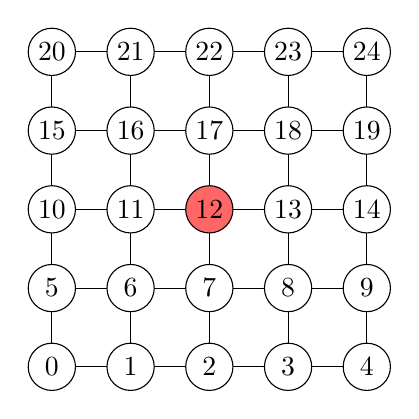
\begin{tikzpicture}

      \draw(0,0) -- (0,4);
      \draw(1,0) -- (1,4);
      \draw(2,0) -- (2,4);
      \draw(3,0) -- (3,4);
      \draw(4,0) -- (4,4);

      \draw(0,0) -- (4,0);
      \draw(0,1) -- (4,1);
      \draw(0,2) -- (4,2);
      \draw(0,3) -- (4,3);
      \draw(0,4) -- (4,4);

      \draw[black,fill=white](0,0) circle (0.3) node {0};
      \draw[black,fill=white](1,0) circle (0.3) node {1};
      \draw[black,fill=white](2,0) circle (0.3) node {2};
      \draw[black,fill=white](3,0) circle (0.3) node {3};
      \draw[black,fill=white](4,0) circle (0.3) node {4};

      \draw[black,fill=white](0,1) circle (0.3) node {5};
      \draw[black,fill=white](1,1) circle (0.3) node {6};
      \draw[black,fill=white](2,1) circle (0.3) node {7};
      \draw[black,fill=white](3,1) circle (0.3) node {8};
      \draw[black,fill=white](4,1) circle (0.3) node {9};

      \draw[black,fill=white](0,2) circle (0.3) node {10};
      \draw[black,fill=white](1,2) circle (0.3) node {11};
      \draw[black,fill=red!60](2,2) circle (0.3) node {12};
      \draw[black,fill=white](3,2) circle (0.3) node {13};
      \draw[black,fill=white](4,2) circle (0.3) node {14};

      \draw[black,fill=white](0,3) circle (0.3) node {15};
      \draw[black,fill=white](1,3) circle (0.3) node {16};
      \draw[black,fill=white](2,3) circle (0.3) node {17};
      \draw[black,fill=white](3,3) circle (0.3) node {18};
      \draw[black,fill=white](4,3) circle (0.3) node {19};

      \draw[black,fill=white](0,4) circle (0.3) node {20};
      \draw[black,fill=white](1,4) circle (0.3) node {21};
      \draw[black,fill=white](2,4) circle (0.3) node {22};
      \draw[black,fill=white](3,4) circle (0.3) node {23};
      \draw[black,fill=white](4,4) circle (0.3) node {24};

    \end{tikzpicture}
  \end{center}
  \caption{n=5-ös rács}
  \label{fig:5Racs}
\end{figure}


% \draw [axis line style] (-6.5,0) -- (6.5,0);
% \draw[draw, fill=black] (0,0) circle (0.05);
% \draw[->] (0.1,0.5) -- (1,0.5) node [above=0.1cm] {$\ket{1}$};
% \draw[->] (-0.1,0.5) -- (-1,0.5) node [above=0.1cm] {$\ket{0}$};

